
\documentclass[10pt,conference,compsocconf]{IEEEtran}

\usepackage{cite}


% *** GRAPHICS RELATED PACKAGES ***
%
\ifCLASSINFOpdf
  \usepackage[pdftex]{graphicx}
  % declare the path(s) where your graphic files are
  % \graphicspath{{../pdf/}{../jpeg/}}
  % and their extensions so you won't have to specify these with
  % every instance of \includegraphics
  \DeclareGraphicsExtensions{.pdf,.jpeg,.png}
\else
  % or other class option (dvipsone, dvipdf, if not using dvips). graphicx
  % will default to the driver specified in the system graphics.cfg if no
  % driver is specified.
  \usepackage[dvips]{graphicx}
  % declare the path(s) where your graphic files are
  %\graphicspath{{../figure/}{../result-and-plot/script/}{../result-and-plot/7slaves-result/}}
  % and their extensions so you won't have to specify these with
  % every instance of \includegraphics
  \DeclareGraphicsExtensions{.eps}
\fi

\usepackage[cmex10]{amsmath}

\usepackage{algorithm}
\usepackage{algpseudocode}
%\usepackage{algorithmic}
%\usepackage[boxed,commentsnumbered,ruled]{algorithm2e}
% ALIGNMENT PACKAGES
\usepackage{array}

\usepackage[font=footnotesize]{subfig}

\usepackage{stfloats}

\usepackage{url}


% make changes to the paper visible
\usepackage{changes}


% correct bad hyphenation here
\hyphenation{Map-Reduce}


% Change table caption style
\renewcommand{\thetable}{\arabic{table}}
\renewcommand{\tablename}{Table}
% Change figure caption style
\renewcommand{\figurename}{Figure}



\begin{document}


% paper title
% can use linebreaks \\ within to get better formatting as desired
\title{Memory or Time: Performance Evaluation for Iterative Operation on Hadoop and Spark}


% author names and affiliations
% use a multiple column layout for up to three different
% affiliations
\author{\IEEEauthorblockN{Lei Gu, Huan Li}
\IEEEauthorblockA{State Key Laboratory of Software Development Environment\\
Beihang University, Beijing, China\\
gulei@act.buaa.edu.cn, lihuan@buaa.edu.cn}}
%\and
%\IEEEauthorblockN{Homer Simpson}
%\IEEEauthorblockA{Twentieth Century Fox\\
%Springfield, USA\\
%Email: homer@thesimpsons.com}
%\and
%\IEEEauthorblockN{James Kirk\\ and Montgomery Scott}
%\IEEEauthorblockA{Starfleet Academy\\
%San Francisco, California 96678-2391\\
%Telephone: (800) 555--1212\\
%Fax: (888) 555--1212}}

% conference papers do not typically use \thanks and this command
% is locked out in conference mode. If really needed, such as for
% the acknowledgment of grants, issue a \IEEEoverridecommandlockouts
% after \documentclass

% for over three affiliations, or if they all won't fit within the width
% of the page, use this alternative format:
% 
%\author{\IEEEauthorblockN{Michael Shell\IEEEauthorrefmark{1},
%Homer Simpson\IEEEauthorrefmark{2},
%James Kirk\IEEEauthorrefmark{3}, 
%Montgomery Scott\IEEEauthorrefmark{3} and
%Eldon Tyrell\IEEEauthorrefmark{4}}
%\IEEEauthorblockA{\IEEEauthorrefmark{1}School of Electrical and Computer Engineering\\
%Georgia Institute of Technology,
%Atlanta, Georgia 30332--0250\\ Email: see http://www.michaelshell.org/contact.html}
%\IEEEauthorblockA{\IEEEauthorrefmark{2}Twentieth Century Fox, Springfield, USA\\
%Email: homer@thesimpsons.com}
%\IEEEauthorblockA{\IEEEauthorrefmark{3}Starfleet Academy, San Francisco, California 96678-2391\\
%Telephone: (800) 555--1212, Fax: (888) 555--1212}
%\IEEEauthorblockA{\IEEEauthorrefmark{4}Tyrell Inc., 123 Replicant Street, Los Angeles, California 90210--4321}}

% make the title area
\maketitle


\begin{abstract}
%\boldmath
%an open source implementation of the MapReduce programming model, 

Hadoop is a very popular general purpose framework for many different classes of data-intensive applications. However,  it is not good for iterative operations because of the cost paid for the data reloading from disk at each iteration. As an emerging framework, Spark, which is designed to have a global cache mechanism, can achieve better performance in response time since the in-memory access over the distributed machines of cluster will proceed during the entire iterative process. Although the performance on time has been evaluated for Spark over Hadoop\cite{matei2010}, the memory consumption, another system performance criteria, is not deeply analyzed in the literature. In this work, we conducted extensive experiments for iterative operations to compare the performance in both time and memory cost between Hadoop and Spark. We found that  although Spark is in general faster than Hadoop in iterative operations, it has to pay for more memory consumption. Also, its speed advantage is weakened at the moment when the memory is not sufficient enough to store newly created intermediate results.
\end{abstract}
% Benefited from its characteristics of data cached in memory across machines of cluster

% no keywords
%\begin{IEEEkeywords}
%System performance, Hadoop, Spark, PageRank, running time, memory usage
%\end{IEEEkeywords}

% For peer review papers, you can put extra information on the cover
% page as needed:
% \ifCLASSOPTIONpeerreview
% \begin{center} \bfseries EDICS Category: 3-BBND \end{center}
% \fi
%
% For peerreview papers, this IEEEtran command inserts a page break and
% creates the second title. It will be ignored for other modes.
\IEEEpeerreviewmaketitle



\section{Introduction}
\label{sec:intro}

% no \IEEEPARstart
The rapid development of the Internet has generated vast amount of data that poses big challenges to traditional data processing model. To deal with such challenges, a variety of cluster computing frameworks have been proposed to support large-scale data-intensive applications on commodity machines. MapReduce, introduced by Google\cite{jdean2004} is one such successful framework for processing large data sets in a scalable, reliable and fault-tolerant manner. 
%Dryad\cite{michael2007} takes one step forward and provides support for expressing data processing flows as directed acyclic graphs. Haloop and Twister extend MapReduce to support iterative operations.

Apache Hadoop\cite{url_hadoop} provides an open source implementation of MapReduce.
However, Hadoop is not good for iterative operations which are very common in many applications. MapReduce cannot keep reused data and state information during execution. Thus, MapReduce reads the same data iteratively and materializes intermediate results in local disks in each iteration, requiring lots of disk accesses, I/Os and unnecessary computations. Spark is a MapReduce-like cluster computing framework \cite{url_spark, matei2010}, but it is designed to overcome Hadoop's shortages in iterative operations. Spark introduces a data structure called resilient distributed datasets (RDDs)\cite{matei2012}, through which reused data and intermediate results can be cached in memory across machines of cluster during the whole iterative process. This feature has been proved to effectively improve the performance of those iterative jobs that have low-latency requirements \cite{matei2012}.


Although Spark can achieve tremendous speedup, we suspect the memory cost it has to pay for the introduction of RDDs.  In addition, how to quantify the tradeoff in terms of time and memory for iterative operations is another interesting problem. %In this paper we evaluate the system performance in terms of time and memory between Hadoop and Spark by choosing a typical iterative algorithm PageRank. %We implemented the PageRank algorithm according to the programming models provided by Hadoop and Spark respectively and applied the algorithm to different sizes of graph datasets to compare their running time and memory usage. 

In this paper, we attempted to conduct exhaustive experiments to evaluate the system performance between Hadoop and Spark. We choose a typical iterative algorithm PageRank \cite{page1999} to run for both real and synthetic data sets. Experimental results show: 1) Spark can outperform Hadoop when there is enough memory for Spark in the whole iterative process; 2) Spark is memory consuming. Although input datasets are not that large compared to the whole memory of the cluster, intermediate results generated at each iteration can easily fill up the whole memory of the cluster; 3) Hadoop has better performance than Spark when there is not enough memory to store newly created intermediate results.

% Performance advantage of Spark is weakened to be almost the same as and even worse than Hadoop by insufficient memory.

This paper is organized as follows. Section \ref{sec:sys_ov} provides system overview of Hadoop and Spark. Section \ref{sec:exen} describes our experimental settings. Section \ref{sec:impl} reviews the PageRank algorithm and shows our implementation of PageRank on Hadoop and Spark. Section \ref{sec:results} presents results of our experiment. Related Work is in Section \ref{sec:related_work}. We give our conclusions and future work in Section \ref{sec:concl_fw}.



\section{System Overview}
\label{sec:sys_ov}
%In this section, we provide system overview of Hadoop and Spark and compare the fundamental differences in iterative operations between Hadoop and Spark. Also, we compare Hadoop and Spark in several other aspects.

As a general framework for many different types of big data applications, such as log analysis, web crawler, index building and machine learning, Hadoop\cite{url_hadoop} provides an open source Java implementation of MapReduce. Hadoop is composed of two layers: a data storage layer called Hadoop distributed file system (HDFS) and a data processing layer called Hadoop MapReduce Framework. HDFS is a block-structured file system managed by a single master node.  A processing job in Hadoop is broken down to as many Map tasks as input data blocks and one or more Reduce tasks. An iterative algorithm can be expressed as multiple Hadoop MapReduce jobs. Since different MapReduce jobs cannot keep and share data, frequent used data has to be read from and written back to HDFS many times. Those operations will obviously incur a lot of disk accesses, I/Os and unnecessary computations \cite{jaliya2010} \cite{yingyi2010} \cite{yanfeng2011} during the execution of iterative algorithm.


 
Spark is a novel cluster computing framework that is designed to overcome Hadoop's shortages in iterative operations. Spark does not have its own distributed file system. Instead, it uses Hadoop supported storage systems (e.g, HDFS, HBase) as its input source and output destination.  Spark introduces a data structure called resilient distributed datasets (RDDs)  to cache data. The runtime of Spark consists of a driver and multiple workers. Before an iterative operation, the user's driver program will launch multiple workers. These workers will read data blocks from a distributed file system and cache them in their own memory as partitions of RDD. These partitions form a whole RDD from the view of the driver program. The RDD feature of Spark avoids data reloading from disk at each iteration, which dramatically speeds up the iterative operation. Users can explicitly cache reused data and intermediate results in memory in the form of RDDs and control their partitioning by parameter tuning to optimize data placement. Since RDDs are partitioned across the memory of machines in the cluster, they can be processed in parallel. RDDs are fault-tolerant which means they can be rebuilt if a partition of them is lost. RDDs are read-only, so changes to current RDDs will cause creation of new RDDs.


% The major features of Hadoop and Spark are in Table \ref{tab:feature_hdpspk}.

%   \begin{table*}[!t]
%   \renewcommand{\arraystretch}{1.3}
%   \centering
%   \begin{tabular}{|c|m{1.5cm}<{\centering}|m{1.5cm}<{\centering}|m{1.5cm}<{\centering}|m{1.5cm}<{\centering}|m{2cm}<{\centering}|m{4cm}<{\centering}|m{2cm}<{\centering}|}
%   \hline
%   \bfseries Platform & \bfseries Programming Language & \bfseries Independence of Storage & \bfseries Parallelism & \bfseries Scalability & \bfseries Fine-grained Fault-tolerance & \bfseries Expressivilty & \bfseries Delarative Query Language Support\\
%   \hline
%   Hadoop & Java & Yes & Yes & Yes & Yes & Can express many statistical and learning algorithms. & Pig Latin, HiveQL \\
%   \hline
%   Spark & Scala & Yes & Yes & Yes & Yes  &The operators provided by RDDs can not only express MapReduce models, but also express models like DryadLINQ, SQL and Pregel. & Shark \\
%   \hline
%   \end{tabular}
%   \caption{Features of Hadoop and Spark}
%   \label{tab:feature_hdpspk}
%   \end{table*}

 


  % \begin{itemize}
  %  %%\item Implementation language: Hadoop-Java, Spark-Scala.
   
  %  \item Programming language: Hadoop-Java, Spark-Scala. Scala integrates features of object-oriented and functional languages which makes applications implementation in Spark more concise and elegant. %%Algorithms implemented by Spark is always shorter than those implemented by Hadoop.
   
  %  \item Independence of storage: Both platforms are independent from underlying storage layers.  %%Spark can read data from any Hadoop input source, e.g., HDFS, HBase, using Hadoop's existing input plugin APIs. 
   
  %  \item Parallelism: In Hadoop, a job can be divided into multiple small Map and Reduce tasks running in machines of a cluster which provide high parallelism. In Spark, a job can launch multiple workers in machines of a cluster which can also provide high parallelism. 
   
  %  \item Fine-grained fault-tolerance: both platforms can re-run failed or slow tasks on other nodes.
   
  %  \item Expressivity: MapReduce in Hadoop can express many statistical and learning algorithms. While RDDs in Spark are more expressive. The operators provided by RDDs can not only express MapReduce models, they can also express models like DryadLINQ, SQL and Pregel.
   
  %  \item High Level language (Delarative Query Language) support: Hadoop has Pig Latin and HiveQL, while Spark has Shark.
  % \end{itemize}




%HDFS is inefficient for handling small files. Hadoop MapReduce is a batch-based architecture which means it does not lend itself to use cases which needs real-time data access.

%The framework is memory based and also retains the reliability and fault tolerance of MapReduce.


\section{Experimental Environment}
\label{sec:exen}
%This section presents our experimental cluster architecture and shows graph datasets used in the experiment.

\subsection{Cluster Architecture}
The experimental cluster is composed of eight computers. One of them is designated as master, and the other seven as slaves. We use the operating system Ubuntu 12.04.2 (GNU/Linux 3.5.0-28-generic x86 64) for all the computers. Table \ref{tab:machine_info} shows the hostname, machine modal, IP address, CPU and memory information of the eight computers mentioned above.  All of the eight computers are in the same Local Area Network and connected by a H3C S5100 switch whose port rate is 100Mbps. All of the eight computers have 4 cores, but master and slaves have different frequencies. %From the table we can also see that the master has more total amount of memory than slaves, and that the amount of free memory of each host is about 3400 MB.

% master: 3.10 GHz  1600 MHz
% slave1: 2.83 GHz  2825 MHz
% slave2: 2.83 GHz  2825 MHz
% slave3: 2.83 GHz  2825 MHz
\begin{table*}[!t]
\renewcommand{\arraystretch}{1.5}
\centering
\begin{tabular}{|c|c|c|c|c|c|}
\hline
\bfseries Hostname & \bfseries Machine Modal & \bfseries IP & \bfseries CPU Info & \bfseries Total Memory & \bfseries Free Memory\\
\hline
master & Dell Optiplex 790 & 192.168.2.99 & Intel i5 3.10GHz & 3910MB & \~{}3400MB\\
\hline
slave0 & Dell Optiplex 980 & 192.168.2.100 & Intel i5 3.20GHz & 3816MB & \~{}3400MB\\
\hline
slave1-slave6 &  Dell Optiplex 960 & 192.168.2.101-192.168.2.106 & Intel 2 Quad 2.83GHz & 3825MB & \~{}3400MB\\
\hline
\end{tabular}
\caption{Information of machines in the cluster.}
\label{tab:machine_info}
\end{table*}


Apache Mesos\cite{hindman2011, url_mesos} is a cluster manager that provides efficient resource isolation and sharing across distributed frameworks. It can run Hadoop, Spark, MPI, Hypertable and other frameworks. We use Mesos to manage the resources of our experimental cluster. Fig. \ref{fig:cluster-architec} shows the architecture, where  each slave contributes 4 CPU cores and 3GB memory to Mesos. So the total resources managed by Mesos are 28 CPU cores and 21 GB memory. When a job is submitted to Hadoop or Spark, Mesos will allocate resources to it according to its demanding needs. 

We use Mesos 0.9.0, Hadoop 0.20.205.0 and Spark 0.6.1 for all the experiments shown below, since  Mesos 0.9.0 and Spark 0.6.1 are relatively new stable release. Although Hadoop 1.1.2 \footnote{We also install Hadoop 1.1.2 separately to repeat the experiment, and find that the new version Hadoop does have performance improvement and the improvement is a constant under different graph datasets. Due to space limitations, we will not show the results here.} is the most recent stable release as of writing this paper, only Hadoop 0.20.205.0 is ported to run on mesos. We choose Hadoop 0.20.205.0 in order to let Spark and Hadoop share the same experimental conditions.
\begin{figure}[!t]
\centering
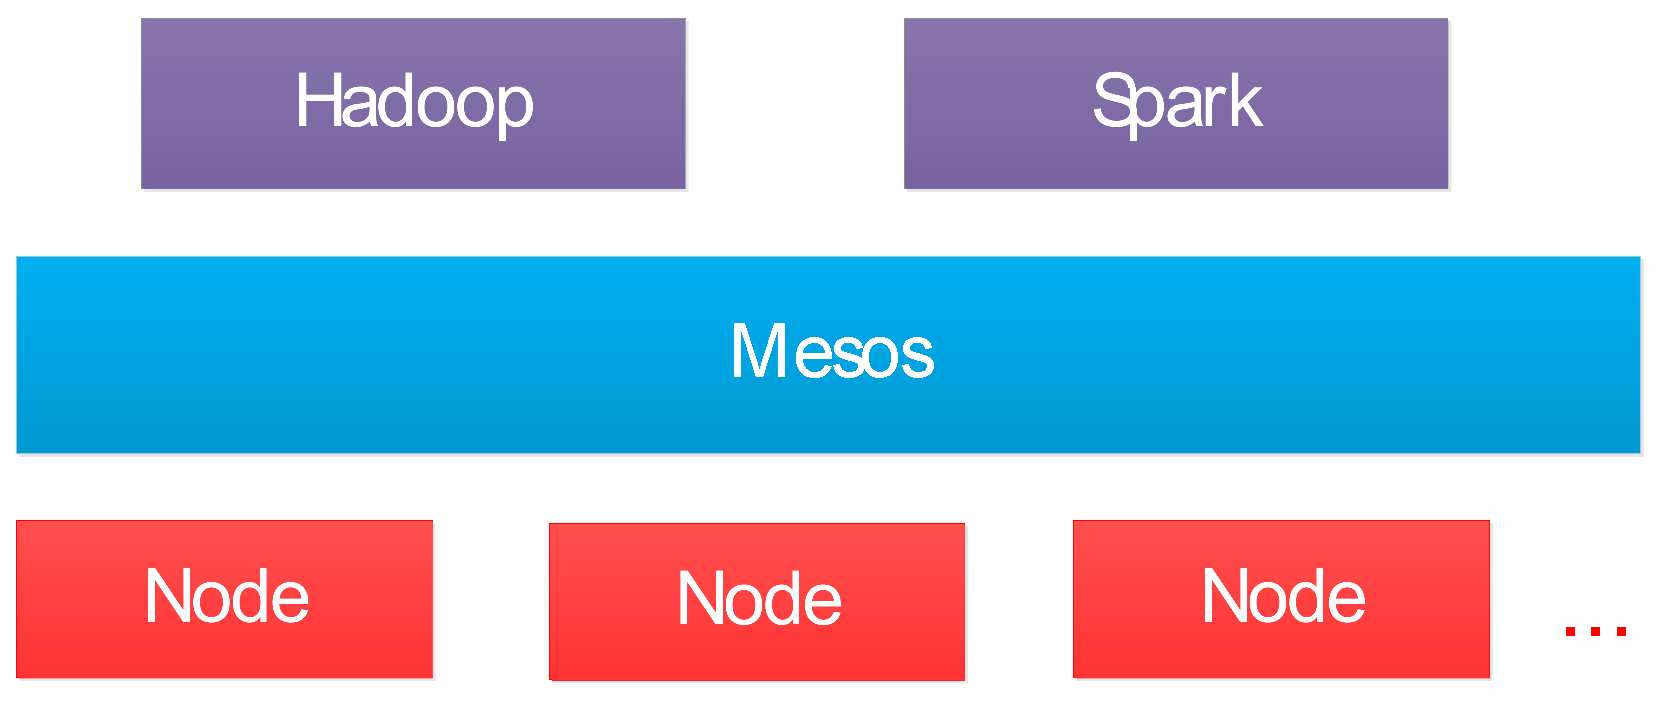
\includegraphics[width=0.4\textwidth]{figures/cluster-architect.eps}
\caption{Cluster architecture.}
\label{fig:cluster-architec}
\end{figure}


\subsection{Dataset Description}
\label{subsec:dataset_des}

Data size and data connectedness are two important properties of a specific dataset. In terms of graph dataset, the number of nodes reflects its size and the number of edges reflects its internal connectedness. These two properties have great impact on the running time and memroy usage of the PageRank algorithm. Also, PageRank run on directed graphs. So we will choose directed graphs with different node number and edge number as our experimental datasets.


We choose five real graph datasets and generate five synthetic graph datasets to do comparative experiments. Table \ref{tab:attribs_graphs} lists these ten graph datasets. They are all in the format of edge list. To be more specific, each line in the file is a [src ID] [target ID] pair separated by whitespace. The first four real graph datasets come from SNAP\cite{url_snap} and the fifth one is obtained from \cite{url_twitter_dataset}. We choose them because they are directed, have significant differences in size and are in different application fields. The five synthetic graph datasets are generated by stochastic Kronecker graph generator. According to \cite{jurij2005}, the Kronecker generator can generate graphs with similar properties as real-world graphs, such as heavy tails for in- and out-degree distribution, small diameters, and densification and shrinking diameters over time. We utilize the Kronecker generator provided in SNAP\cite{url_snap}. We first create a radom seed graph with only two nodes, then pass it to the generator and make it iterate the specified number of times to get the expected size of synthetic graph we need. We will use the name attribute to reference the specific graph dataset in the following description.

%More specifically, each line in a graph dataset file is in the form of ``$n_i\;n_j$'' which represents a directed arc from node $i$ to node $j$. 

%In order to observe these two properties more intuitively, we plot them in Fig. \ref{fig:node_edge_number}. From Fig. \ref{fig:node_edge_number} we can see that the node numbers gradually increases from wiki-Vote to kronecker2 except web-Google which is slighly bigger than its subsequent web-BerkStan and the edge numbers exhibit exponential increasing trend from wiki-vote to kronecker2.

%We use longest shortest path as the diameter of a graph. The fifth column of Table \ref{tab:attribs_graphs} gives the diameters of different graphs. As the graph size and connectedness increases, the graph diameter exhibits a shrinking trend except web-Stanford and web-BerkStan.

%From Fig. \ref{fig:wiki-Votedegreedist} to Fig. \ref{fig:kronecker2degreedist}, We also plot the in-degree and out-degree distributions of different graphs. The degree distributions of all the graphs have heavy tails. The in-degree distributions of all the graphs meet the power law distribution. For out-degree distributions, all the graphs apart from web-Stanford and web-BerkStan meet the power law distribution.

%From the properties of diameters and degree distributions of different graphs, we can conclude that the two graphs web-Stanford and web-BerkStan are different from the other graphs.


\begin{table*}[!t]
\renewcommand{\arraystretch}{1.5}
\centering
\begin{tabular}{|c|c|c|c|c|}
\hline
\bfseries Name & \bfseries File Size & \bfseries Nodes & \bfseries Edges & \bfseries Description\\
\hline
wiki-Vote & 1.0 MB & 7,115 & 103,689 & Wikipedia who-votes-on-whom network\\
\hline
soc-Slashdot0902 & 10.8 MB & 82,168 & 948,464 & Slashdot social network from February 2009\\
\hline
web-Google & 71.9 MB & 875,713 & 5,105,039 & Web graph from Google\\
\hline
cit-Patents & 267.5 MB & 3,774,768 & 16,518,948 & Citation network among US Patents\\
\hline
Twitter & 1.3 GB & 11,316,811 & 85,331,845 & Twitter social network on who follows whom network\\
\hline
kronecker19 & 40 MB & 416,962 & 3,206,497 & Synthetic graph generated by Kronecker generator
 with 19 iterations.\\
\hline
kronecker20 & 89MB & 833,566 & 7,054,294 & Synthetic graph generated by Kronecker generator
 with 20 iterations.\\
\hline
kronecker21 & 209MB & 1,665,554 & 15,519,448 & Synthetic graph generated by Kronecker generator
 with 21 iterations.\\
\hline
kronecker22 & 479MB & 3,330,326 & 34,142,787 & Synthetic graph generated by Kronecker generator
 with 22 iterations.\\
\hline
kronecker23 & 1.1GB & 6,654,956 & 75,114,133 & Synthetic graph generated by Kronecker generator
 with 23 iterations.\\
\hline
\end{tabular}
\caption{Graph Datasets.}
\label{tab:attribs_graphs}
\end{table*}


% \begin{figure*}[!t]
% \centering
% \includegraphics[width=0.3\textwidth]{dataset/dataset.eps}
% \caption{Plots of nodes number and edges number of different datasets.}
% \label{fig:node_edge_number}
% \end{figure*}



\section{Implementation}
\label{sec:impl}
%This section presents the implementation of PageRank algorithm on Hadoop and Spark platforms.

\subsection{PageRank Overview}
The basic idea behind PageRank is that a node which is linked to by a large number of high quality nodes tends to be of high quality. In order to measure a node's quality, an authoritive value called PageRank value can be assigned to each node in the whole graph. Formally, the PageRank $P$ of a node $n$ is defined as follows:

%So in the graph context, nodes that have high PageRank values are those that have high in-degrees and are linked to by other nodes with high PageRank values.

%The random surfer model \cite{page1999} can be utilized to better understand PageRank. PageRank was used to simulate where Web surfers, starting at a random page, would tend to congregate if they followed randomly chosen outlinks from the page at which they were currently located, and this process were allowed to iterate many times. Pages that would have a large number of surfers were considered more ``important'' than pages that would rarely be visited. In a nutshell, PageRank value represents the likelyhood that a random walk over the link structure will arrive at a particular node. 

\begin{equation}
P(n) = \sum_{m \in L(n)} \frac{P(m)}{C(m)} \label{eq:pr_1}
\end{equation}
where $L(n)$ is the set of nodes that link to $n$, $P(m)$ is the PageRank of node $m$, $C(m)$ is the out-degree of node $m$.

%Formula \ref{eq:pr_1} is actually a simplified version of PageRank definition and is only suited for a strongly connected graph. However, graphs in real world are not that perfect. So, the simplified version of PageRank needs to be modified to deal with some special structures of real graphs.

There are two anomalies we need to prevent. The first one involves the structure called $spider\;trap$ which are group of nodes that have no links out of the group. This will cause the PageRank calculation to place all the PageRank within the spider trap. The second one is related to $dangling\;nodes$ which are nodes in the graph that have no outlinks. The total PageRank mass will not be conserved due to dangling nodes. 
%PageRank values at dangling nodes will leak out of the graph and the total PageRank mass will not be conserved.


To deal with the first problem, a random jump factor $\alpha$ can be added to the Formula \ref{eq:pr_1}. According to \cite{monica2005}, the second problem can be solved by redistributing PageRank mass ``lost'' at dangling nodes across all nodes in the graph evenly. That is, for node $n$, its current PageRank value $P(n)$ is updated to the final PageRank value $P(n)'$ according to the following formula:
\begin{equation}
P(n)' = \alpha (\frac{1}{|G|}) + (1 - \alpha) (\frac{l}{|G|} + P(n)) \label{eq:pr_2}
\end{equation}
where $|G|$ is the total number of nodes in the graph, $\alpha$ is the random jump factor, $l$ is the total PageRank mass ``lost'' at dangling nodes.


\subsection{PageRank on Hadoop}
Our PageRank implementation on Hadoop references the idea in\cite{jimmy2010}. The basic process of each PageRank iteration can be divided into two Hadoop MapReduce jobs.

%The first job corresponds to Formula \ref{eq:pr_1}. 
In the first job, each node $m$ first divides its current PageRank value $P(m)$ evenly by $C(m)$, the number of nodes $m$ links to and passes each share to them separately. This distribution process is implemented by a map function. Then each node $n$ sums up all PageRank contributions that have been passed to it and gets its new PageRank value $P(n)$. This aggregation process is implemented by a reduce funtion. The first job implementation of PageRank iteration on Hadoop is shown in Algorithm \ref{algo:hadoop_pr_job1}. 


\begin{algorithm}[!t]
\caption{First job of Hadoop PageRank iteration}
\label{algo:hadoop_pr_job1}
\begin{algorithmic}[1]
\Function {Map}{$m$, $<curPR, NeighborList>$} 
    \State $contribution \leftarrow \frac{curPR}{|NeighborList|}$ 
    \ForAll {$n \in NeighborList$}
      \State $EMIT(n, contribution)$ \Comment PageRank distribution
    \EndFor    
  \State $EMIT(m, NeighborList)$   
\EndFunction
\end{algorithmic}
\;\;\;
\begin{algorithmic}[1]
\Function {Reduce}{$n$,$<ContributionList,NeighborList>$}  
  \State $p \leftarrow 0$
  \ForAll {$c \in ContributionList$}
    \State $p = p + c$  \Comment PageRank aggregation
  \EndFor
  \State $EMIT(m, <p, NeighborList>)$
\EndFunction
\end{algorithmic}
\end{algorithm}


Before the second job, the total PageRank loss $l$ at dangling nodes needs to be calculated. We get the total PageRank loss $l$ by first summing up the PageRank value each node has after the first job and then using one minus this sum.

%The second job corresponds to Formula \ref{eq:pr_2}. 
In the second job, each node $n$ updates its current PageRank value $P(n)$ to $P(n)'$ according to Formula \ref{eq:pr_2}. The PageRank loss $l$ computed before can then be evenly distributed to all the nodes in the graph. The random jump factor $\alpha$ can also be added at each node. The second job is implemented by a map function only job. Algorithm \ref{algo:hadoop_pr_job2} gives the second job implementation of PageRank iteration on Hadoop.
\begin{algorithm}[!t]
\caption{Second job of Hadoop PageRank iteration}
\label{algo:hadoop_pr_job2}
\begin{algorithmic}[1]
\Function {Map}{$n$, $<p, NeighborList>$}
    \State $l \leftarrow$ PageRank loss\;
    \State $N \leftarrow$ number of nodes in the graph
    \State $\alpha \leftarrow$ random jump factor    
    \State $p' = \alpha\times\frac{1}{N} + (1 - \alpha) \times (\frac{l}{N} + p)$
    \Comment PageRank loss distribution and random jump factor treatment
    \State $curPR = p'$     
    \State $EMIT(n, <curPR, NeighborList>)$    
\EndFunction
\end{algorithmic}
\end{algorithm}

% {\bf 
% Phase 1 deals with PageRank distribution and aggregation at each node. Each node passes its PageRank contributions to the nodes that it is connected to. This distribution process can be implemented by a Mapper. To conclude phase 1, each node sums up all PageRank contributions that have been passed to it. This aggregation process can be implemented by a Reducer. 

% Extra operations need to be done to prepare for phase 2. The operations are to read the result files generated by Phase 1 line by line to extract and sum all the PageRank masses each node gets. Since dangling nodes will not distribute their PageRanks to other nodes because of their zero out-degree, we can get the total of PageRank loss at all dangling nodes in the graph by using one minus the sum. The PageRank loss will be used in phase 2.

% Phase 2 deals with the PageRank loss and the random jump factor. The PageRank loss computed before can then be evenly distributed to all the nodes in the graph. The random jump factor can also be added at each node. Phase 2 can be implemented by a Mapper only job. 
% }

% Hadoop provides an open source implementation of MapReduce programming model. This subsection gives a detailed description of our implementation of PageRank on Hadoop platform using the interfaces exposed by Hadoop platform.

% There are four major components in MapReduce: $Mapper$, $Reducer$, $Partitioner$, and $Combiner$. $Mapper$ is used for data filtering and transformation. $Reducer$ is used for global data aggregation. $Partitioner$ provides some criteria to distribute data generated by Mapper to a specific Reducer. $Combiner$ is used for local aggregation. Of all the four components, $Mapper$ and $Reducer$ are at the core of MapReduce. We implement these two components and use the default implementation of the other components provided by Hadoop.

% To implement PageRank algorithm on Hadoop platform, two steps need to be gone through. The first one is to represent graph with adjacency list and meanwhile initialize
% PageRank value for each node. The second one is PageRank iterations. Below are detailed descriptions of the two steps in MapReduce programming model.

% \subsubsection{Step 1. Data preprocessing}

% Each line in the original graph dataset file is in the form of ``$n_i\;n_j$'', which represents a directed edge from node $i$ to node $j$. In step 1, we need to collect all the nodes each node links to and meanwhile initialize the PageRank value for each node. For example, if node A links to node B, C, and D, there should be three lines in the form of ``A B'', ``A C'' and ``A D'' scattered in the original graph dataset file. In step 1, we need to collect nodes B, C, D for node A, and generate a single line in the form of ``A B,C,D''. Meanwhile, we need to initialize a PageRank value for node A. So the line would become ``A oldPR,curPR,B,C,D''. In the initialzation process, oldPR is assigned to 0 and curPR is assigned to $\frac{1}{N}$ where $N$ is the number of nodes in a specific graph dataset.

% Pseudo-code of data preprocessing in MapReduce is shown in Algorithm \ref{algo:hadoop_datapre_mapper} and \ref{algo:hadoop_datapre_reducer}. Note that in all the algorithms we present key-value pair is represented in the form of ``$K \rightarrow V$''.

% % data preprocessing Mapper
% \begin{algorithm}[!t]  
%   \caption{data preprocessing: Mapper}
%   \label{algo:hadoop_datapre_mapper}
%   \dontprintsemicolon
%   \SetKwFunction{MAP}{map}\SetKwFunction{REDUCE}{reduce}\SetKwFunction{EMIT}{emit}
%   \SetKwInOut{Input}{input}\SetKwInOut{Output}{output}
%   \Input{line offset $\rightarrow$ node$i$ node$j$}
%   \Output{node$i$ $\rightarrow$ node$j$}  
%   \BlankLine
%   \MAP{line offset, node$i$ node$j$}\;
%       \Indp \Indp 
%       $K \leftarrow$ node$i$\;
%       $V \leftarrow$ node$j$\;
%       \EMIT{$K$, $V$}\;
% \end{algorithm}

% % data preprocessing Reducer
% \begin{algorithm}[!t]
%   \caption{data preprocessing: Reducer}
%   \label{algo:hadoop_datapre_reducer}
%   \dontprintsemicolon
%   \SetKwFunction{MAP}{map}\SetKwFunction{REDUCE}{reduce}\SetKwFunction{EMIT}{emit}
%   \SetKwInOut{Input}{input}\SetKwInOut{Output}{output}
%   \Input{node$i$ $\rightarrow$ $<$node$x$,node$y$,node$z$\ldots{}$>$}
%   \Output{node$i$ $\rightarrow$ $<0,\frac{1}{N}$,node$x$,node$y$,node$z$\ldots{}$>$}
%   \tcp{N is the total number of nodes in the graph}
%   \BlankLine
%   \REDUCE{node$i$, $<$node$x$,node$y$,node$z$\ldots{}$>$}\;
%        \Indp \Indp
%         $K \leftarrow$ node$i$\;
%         $V \leftarrow$ $<0,\frac{1}{N}$,node$x$,node$y$,node$z$\ldots{}$>$\;
%         \EMIT{$K$, $V$}\;
% \end{algorithm}

% \subsubsection{Step 2. PageRank iteration}
% After data preprocessing, we can proceed to perform PageRank iteration. Since it is iterative operation, the output format of previous iteration should be consistent with the input format of next iteration. 

% The basic process of each iteration can be divided into two phases each of which corresponds to a MapReduce job. We call the first phase phase 1 and the second phase 2.

% Phase 1 deals with PageRank distribution and aggregation at each node. Each node passes its PageRank contributions to the nodes that it is connected to. Since PageRank is a probability distribution, we can think of this as spreading probability mass to neighbors via outgoing links. This distribution process can be implemented by a Mapper which is shown in Algorithm \ref{hadoop_pr_phase1_mapper}. To conclude phase 1, each node sums up all PageRank contributions that have been passed to it. This aggregation process can be implemented by a Reducer which is shown in Algorithm \ref{hadoop_pr_phase1_reducer}. 

% Extra operations need to be done to prepare for phase 2. The operations are to read the result files generated by Phase 1 line by line to extract and sum all the PageRank masses each node gets. Since dangling nodes will not distribute their PageRanks to other nodes because of their zero out-degree, we can get the total of PageRank loss at all dangling nodes in the graph by using one minus the sum. The PageRank loss will be used in phase 2.

% Phase 2 deals with the PageRank loss and the random jump factor. The PageRank loss computed before can then be evenly distributed to all the nodes in the graph. The random jump factor can also be added at each node. Phase 2 can be implemented by a Mapper which is shown in Algorithm \ref{hadoop_pr_phase2_mapper}.

% Pseudo-code of PageRank iteration in MapReduce is shown in Algorithm \ref{hadoop_pr_phase1_mapper}, \ref{hadoop_pr_phase1_reducer} and \ref{hadoop_pr_phase2_mapper}. Note that the iteration stops when the stopping criteria is met as discussed earlier.

% % PageRank iteration Mapper
% \begin{algorithm}[!t]
%    \caption{PageRank iteration phase 1: Mapper}
%    \label{hadoop_pr_phase1_mapper}
%    \dontprintsemicolon
   
%    \SetKwFunction{MAP}{map}
%    \SetKwFunction{REDUCE}{reduce}
%    \SetKwFunction{EMIT}{emit}
%    \SetKwInOut{Input}{input}
%    \SetKwInOut{Output}{output}

%    \Input{node$i$ $\rightarrow$ $<$oldPR,curPR,node$x$,node$y$,node$z$\ldots{}$>$}
%    \Output{node$i$ $\rightarrow$ curPR}
%    \Output{node$x$ $\rightarrow$ PR contribution from node$i$;\\node$y$ $\rightarrow$ PR contribution from node$i$;\\node$z$ $\rightarrow$ PR contribution from node$i$;\\ \ldots}
%    \Output{node$i$ $\rightarrow$ $<$node$x$,node$y$,node$z$\ldots{}$>$}
%    \BlankLine
%    \MAP{node$i$, $<$oldPR,curPR,node$x$,node$y$,node$z$\ldots{}$>$}\;
%       \Indp \Indp
%       $K1 \leftarrow$ node$i$\;
%       $V1 \leftarrow curPR$\;
%       \EMIT{$K1$, $V1$}\;
%       \BlankLine
%       $L \leftarrow$ $<$node$x$,node$y$,node$z$\ldots{}$>$\;
%       $N \leftarrow$ length of $L$\;
%       $contrib \leftarrow \frac{curPR}{N}$\;      
%       \lForEach{node in $L$}{\\
%         \Indp \Indp
%         $K2 \leftarrow$ node\;
%         $V2 \leftarrow contrib$ \;
%         \EMIT{$K2$, $V2$}\; 
%       }\;
%       \BlankLine
%       \Indm \Indm
%       $K3 \leftarrow$ node$i$\;
%       $V3 \leftarrow  L$\;
%       \EMIT{$K3$, $V3$}\;
% \end{algorithm}


% % PageRank iteration Reducer
% \begin{algorithm}[!t]  
%    \caption{PageRank iteration phase 1: Reducer}
%    \label{hadoop_pr_phase1_reducer}
%    \dontprintsemicolon
%    \SetKwFunction{MAP}{map}\SetKwFunction{REDUCE}{reduce}\SetKwFunction{EMIT}{emit}
%    \SetKwInOut{Input}{input}\SetKwInOut{Output}{output}

%     \Input{node$i$ $\rightarrow$ curPR}
%     \Input{node$i$ $\rightarrow$ $<$contrib1, contrib2, contrib3\ldots{}$>$}
%     \Input{node$i$ $\rightarrow$ $<$node$x$,node$y$,node$z$\ldots{}$>$}
%     \Output{node$i$ $\rightarrow$ $<$oldPR,contribSum,node$x$,node$y$,node$z$\ldots{}$>$}

%     \BlankLine
%     \REDUCE{node$i$, $Input$}\;
%       \Indp \Indp
%       $K \leftarrow$ node$i$\;
%       \If{$Input$ in the form of node$i$ $\rightarrow$ curPR}{
%         $V1 \leftarrow curPR$\;
%       }\;
%       \If{$Input$ in the form of node$i$ $\rightarrow$ $<$contrib1, contrib2, contrib3\ldots{}$>$}{
%         $CList \leftarrow$ $<$contrib1, contrib2, contrib3\ldots{}$>$\;
%         $V2 \leftarrow 0$\;
%         \lForEach{contrib in $CList$}{\\
%           \Indp \Indp
%           $V2 = V2 + $ contrib\;
%         }\;               
%       }\;
%       \If{$Input$ in the form of node$i$ $\rightarrow$ $<$node$x$,node$y$,node$z$\ldots{}$>$}{
%         $V3 \leftarrow$ $<$node$x$,node$y$,node$z$\ldots{}$>$\;
%       }\;
%       \EMIT{$K$, $<V1,V2,V3>$}\;
% \end{algorithm}



% \begin{algorithm}[!t]
%    \caption{PageRank iteration phase 2: Mapper}
%    \label{hadoop_pr_phase2_mapper}
%    \dontprintsemicolon
%    \SetKwFunction{MAP}{map}\SetKwFunction{REDUCE}{reduce}\SetKwFunction{EMIT}{emit}
%    \SetKwInOut{Input}{input}\SetKwInOut{Output}{output}

%    \Input{node$i$ $\rightarrow$ $<$oldPR,contribSum,node$x$,node$y$,node$z$\ldots{}$>$}
%    \Output{node$i$ $\rightarrow$ $<$oldPR,curPR,node$x$,node$y$,node$z$\ldots{}$>$}   
%    \BlankLine
%    \MAP{node$i$, $<$oldPR,contribSum,node$x$,node$y$,node$z$\ldots{}$>$}\;
%       \Indp \Indp
%       $K1 \leftarrow$ node$i$\;
%       $p \leftarrow$ contribSum\;
%       $m \leftarrow$ PageRank loss\;
%       $N \leftarrow$ number of nodes in the graph\;      
%       $p' = \alpha\times\frac{1}{N} + (1 - \alpha) \times (\frac{m}{N} + p)$\;
%       $V1 \leftarrow$ $<$oldPR,$p'$,node$x$,node$y$,node$z$\ldots{}$>$
%       \EMIT{$K1$, $V1$}\;      
% \end{algorithm}

\subsection{PageRank on Spark}
The authors who invent Spark provide a simple implementation of PageRank on Spark. But their implementation did not consider the dangling nodes in the graph. There are actually a large number of dangling nodes in both real and synthetic graphs. Dealing with dangling nodes is a necessary step, so we reimplement PageRank on Spark by taking into account the dangling nodes in order to make the PageRank implementation on Hadoop and Spark be consistent and practical.

All the iterative operations can be implemented in a Spark driver. Each iteration includes four steps. The first step distributes the PageRank value of each node to its neighbors using the join and flatMap transformation. The second step does PageRank aggregation for each node using reduceByKey transformation. In the third step, PageRank loss at dangling nodes is computed. The fourth step deals with PageRank loss distribution and random jump factor. 


% Spark revolves around the concept of $resilient\;distributed\;dataset$ (RDD), which is a fault-tolerant collection of elements that can be operated on in parallel. There are currently two types of RDDs: $parallelized\;collections$, which take an existing Scala collection and run functions on it in parallel, and $Hadoop\;datasets$, which run functions on each record of a file in Hadoop distributed file system or any other storage system supported by Hadoop.

% Iterative operations can be implemented by Spark jobs. Before each Spark job, dataset of interest can first be loaded from disk into the memory and represented as RDD across machines of the whole cluster. Then the job can be run with data (in RDD form) kept in memory for the whole iterative process. After job running, results can be written to disk. Fewer disk accesses and memory based process contribute to its performance improvements.

% RDDs support two types of operations: $transformations$, which create a new dataset from an existing one, and $actions$, which return a value to the driver program after running a computation on the dataset. Some common transformations and actions supported by RDD and their meanings are listed in Table \ref{tab:rdd_transformations} and Table \ref{tab:rdd_actions} separately. 

% \begin{table*}[!t]
% \renewcommand{\arraystretch}{1.3}
% \centering
% \begin{tabular}{|c|p{10cm}|}
% \hline
% \bfseries Transformation & \bfseries Meaning\\
% \hline
% map($func$) & Return a new distributed dataset formed by passing each element of the source through a function $func$.\\
% \hline
% flatMap($func$) & Similar to map, but each input item can be mapped to 0 or more output items (so $func$ should return a Seq rather than a single item).\\
% \hline
% reduceByKey($func$) & When called on a dataset of (K, V) pairs, returns a dataset of (K, V) pairs where the values for each key are aggregated using the given reduce function.\\
% \hline
% join($otherDataset$) & When called on datasets of type (K, V) and (K, W), returns a dataset of (K, (V, W)) pairs with all pairs of elements for each key.\\
% \hline
% \end{tabular}
% \caption{Common transformations supported by RDD.}
% \label{tab:rdd_transformations}
% \end{table*}

% \begin{table*}[!t]
% \renewcommand{\arraystretch}{1.3}
% \centering
% \begin{tabular}{|c|p{10cm}|}
% \hline
% \bfseries Action & \bfseries Meaning\\
% \hline
% reduce($func$) & Aggregate the elements of the dataset using a function $func$ (which takes two arguments and returns one). The function should be associative so that it can be computed correctly in parallel.\\
% \hline
% count() & Return the number of elements in the dataset.\\
% \hline
% saveAsTextFile($path$) & Write the elements of the dataset as a text file (or set of text files) in a given directory in the local filesystem, HDFS or any other Hadoop-supported file system. Spark will call toString on each element to convert it to a line of text in the file.\\
% \hline
% \end{tabular}
% \caption{Common actions supported by RDD.}
% \label{tab:rdd_actions}
% \end{table*}

% To implement PageRank algorithm on Spark platform, two steps are also required. The first one is to represent the graph with adjacency list which is similar to that of Hadoop but without PageRank initialization. This step can be implemented by making small modifications to that of Hadoop. The second one is PageRank iterations. we mainly focus on the implementation of the second step.

% Before iteration, we need to compute the number of nodes in the graph and construct two RDDs. The first RDD is a pair list of (node, neighbors) with node standing for the id of a specific node in the graph and neighbors standing for a list of ids this node links to. The second RDD is a pair list of (node, rank) with node also standing for the id of a specific node in the graph and rank standing for the PageRank value of this node and being set to 1/N at the beginning.

% Then we can proceed to do PageRank iterations. Each iteration includes four steps. The first step distributes the PageRank value of each node to its neighbors using the join and flatMap transformation. The second step does PageRank aggregation for each node using reduceByKey transformation. In the third step, PageRank loss at dangling nodes is computed. The fourth step deals with PageRank loss distribution and random jump factor. 

% After PageRank iterations, the rank for each node can be saved using saveAsTextFile action.

The detailed PageRank implementation on Spark is shown in Algorithm \ref{algo:spark_pr}.

\begin{algorithm}[!t]
\caption{Spark PageRank iteration}
\label{algo:spark_pr}
\begin{algorithmic}[1]
\State val N = ...    \Comment number of nodes in the graph
\State val links = ... \Comment RDD of (node, neighbors) pairs
\State var ranks = ... \Comment RDD of (node, rank) pairs
\For{$i=0$ to ITERATIONS}
\State val contribs = links.join(ranks).flatMap(\{ \par
  \hskip\algorithmicindent case (node, (neighbors, rank)) $=>$ \par
  \hskip\algorithmicindent \hskip\algorithmicindent neighbors.map( \par
  \hskip\algorithmicindent \hskip\algorithmicindent \hskip\algorithmicindent neighbor $=>$ \par
  \hskip\algorithmicindent \hskip\algorithmicindent \hskip\algorithmicindent \hskip\algorithmicindent(neighbor, rank/neighbors.size)) \par
  \})  \Comment PageRank distribution
\State ranks = contribs.reduceByKey($\_ + \_$) \par \Comment PageRank aggregation
\State dMass = ranks.reduce( \par
  \hskip\algorithmicindent ($p1$, $p2$) $=>$ ("dm", $p1.\_2 + p2.\_2$) \par
  ).\_2
\State lMass = 1 - dMass  \Comment PageRank loss computation
\State ranks = ranks.mapValues( \par
   \hskip\algorithmicindent $v => \alpha\times\frac{1}{N} + (1 - \alpha) \times (\frac{lMass}{N} + v)$ \par
   ) \Comment PageRank loss distribution and random jump factor treatment
\EndFor 
\State ranks.saveAsTextFile(...)
\end{algorithmic}
\end{algorithm}

% % Spark PageRank iteration
% \begin{algorithm}[!t]
% \caption{Spark PageRank iteration}
% \label{algo:spark_pr}
% \begin{algorithmic}
% \STATE val N =  ;   //number of nodes in the graph
% \STATE val links =  ;  // RDD of (node, neighbors) pairs
% \STATE var ranks =  ;  // RDD of (node, rank) pairs
% \FOR{$i=0$ to ITERATIONS}
% \STATE val contribs = links.join(ranks).flatMap(\{
%   \STATE case (node, (neighbors, rank)) $=>$ 
%   \STATE neighbors.map(
%     \STATE neighbor $=>$ (neighbor, rank/neighbors.size)
%     \STATE )
% \STATE \}); // PageRank distribution
% \STATE ranks = contribs.reduceByKey($\_ + \_$); // PageRank aggregation
% \STATE dMass = ranks.reduce(($p1$, $p2$) $=>$ ("dm", $p1.\_2 + p2.\_2$)).\_2; 
% \STATE lMass = 1 - dMass; // PageRank loss computation
% \STATE ranks = ranks.mapValues(
% \STATE     $v => \alpha\times\frac{1}{N} + (1 - \alpha) \times (\frac{lMass}{N} + v)$
% \STATE );// PageRank loss distribution and random jump factor treatment
% \ENDFOR 
% \STATE ranks.saveAsTextFile(...)
% \end{algorithmic}
% \end{algorithm}




% %Bagel operates on a graph represented as a distributed dataset of (K, V) pairs, where keys are vertex IDs and values are vertices plus their associated state. In each superstep, Bagel runs a user-specified compute function on each vertex that takes as input the current vertex state and a list of messages sent to that vertex during the previous superstep, and returns the new vertex state and a list of outgoing messages.

% %In the experiment, we use Bagel to implement PageRank, and we only need to implement the user-specified compute function that Bagel exposes to us. The input of the compute function is a specific node containing its current PageRank value combined with a list of PageRank contribution shares from the nodes that link to it. The output is the specific node itself plus a list of contribution shares that will be distributed to the nodes to which this specific node links. So in the compute function, two things need to be done: aggregate the contribution shares from all the followers of a specific node to generate a new PageRank value and evenly distrutes the new value to all its followees. All the other things will be handled by the Bagel utility. Pseudo-code of the user-specified compute function for PageRank is shown in Algorithm 5.

% Spark Bagel PageRank
% \begin{algorithm}[!t]  
%    \caption{Spark PageRank iteration}
%    \dontprintsemicolon
%    \SetKwFunction{COMP}{compute}\SetKwFunction{EMIT}{emit}
%    \SetKwInOut{Input}{input}\SetKwInOut{Output}{output}

%     \Input{node$i$, $<$contrib1, contrib2, contrib3\ldots{}$>$}   
%     \Output{node$i$,$<$(node$x$, share),(node$y$, share), (node$z$, share)\ldots{}$>$}

%     \BlankLine
%     \COMP{node$i$, $<$contrib1, contrib2, contrib3\ldots{}$>$}\;
%       \Indp \Indp        
%       $K \leftarrow$ node$i$\;
%       $CList \leftarrow$ $<$contrib1, contrib2, contrib3\ldots{}$>$\;
%         $V2 \leftarrow 0$\;
%         \lForEach{contrib$i$ in $CList$}{\\
%           \Indp \Indp
%           $V2 = V2 + $ contrib$i$\;
%         }\;
%        \Indm \Indm
%         $N \leftarrow$ number of nodes in the graph\;
%         $V2 = (1 - \alpha) \times V2 + \alpha\times\frac{1}{N}$\;
%         $K.value = V2$\;
%         $LList = K.links$\;
%         $NSList = NULL$\;
%         $S = \frac{V2}{LList.length}$\;
%         \lForEach{node$i$ in $LList$}{\\
%           \Indp \Indp
%           $NSList.add(nodei, S)$\;
%         }\;    
%       \Indm \Indm
%       \EMIT{$K$, $NSList$}\;
% \end{algorithm}


\section{Experiment and Results}
\label{sec:results}
 %This section shows the results of our experiments. We study the scalability of our PageRank implementations on Hadoop and Spark and compare the running time and memory usage of our PageRank implementations on both platforms under different sizes of datasets.


\subsection{Measurement Metrics}
%For a specific graph dataset, we use its number of nodes instead of its number of edges for its size. 
For each dataset we make PageRank run five iterations on Hadoop and Spark respectively, and record the total running time each dataset spends. Meanwhile, when PageRank is running on either Hadoop or Spark, we query and record each slave's system memory usage every second. When it ends, we can plot the temporal change of memory usage for each slave according to the records we have kept.

The purpose of choosing the same iteration number for all the datasets is for fair comparison. The reason why we only show five iterations for all the datasets instead of their convergence iteration time is that five iterations is long enough to help us quantify the time differences between Hadoop and Spark and observe their memory usage patterns.


%We also do preliminary experiments for studying PageRank convergence characteristics which is beyond the scope of this paper.  

\subsection{PageRank Scalability}
%In this subsection, we study the scalability of our PageRank implementations on Hadoop and Spark. For each dataset we make PageRank run five times on both Hadoop and Spark, and record the time each dataset spends.

\begin{figure*}[!t]
    \centering
      \subfloat[Real Graphs]{       
        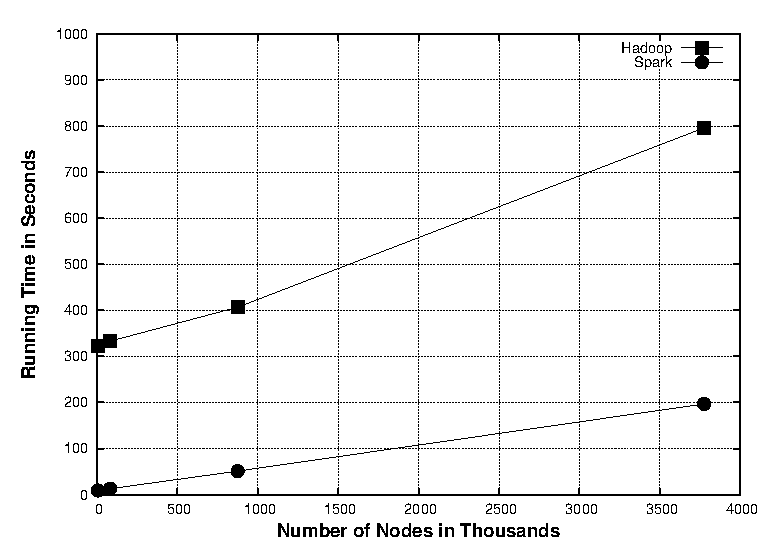
\includegraphics[width=0.4\textwidth]{figures/real-nodes-time.eps}
        }
      \subfloat[Synthetic Graphs]{        
        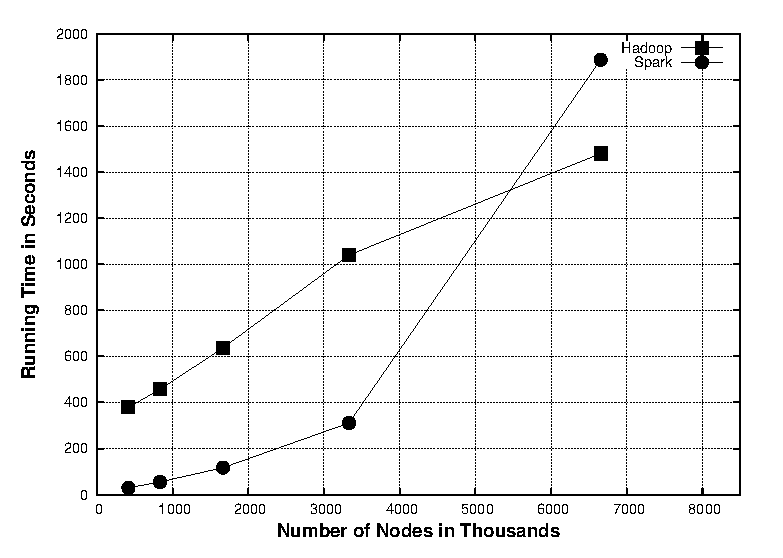
\includegraphics[width=0.4\textwidth]{figures/synthetic-nodes-time.eps}}
    \caption{Scalability comparison.}
    \label{fig:time_vs_size}
\end{figure*}

Fig. \ref{fig:time_vs_size} shows running time versus number of nodes for real and synthetic graph datasets. We have two observations: 1) when datasets are smaller than kronecker22, the PageRank implementations exhibit near-linear scalability on both Hadoop and Spark whether the graphs are real or synthetic; 2) when datasets are larger than kronecker22, slope of Spark line is greater than that of Hadoop line which means that the performance advantage of Spark becomes smaller as the graph size increases.

\subsection{Running Time Comparison}

\begin{figure*}[!t]
\centering
\subfloat[Real Graphs]{
  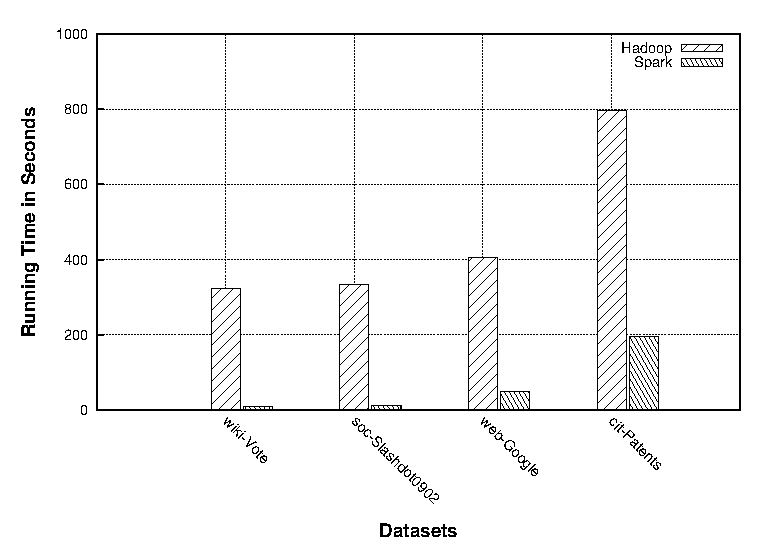
\includegraphics[width=0.4\textwidth]{figures/real-5iterations-time.eps}}
\subfloat[Synthetic Graphs]{
  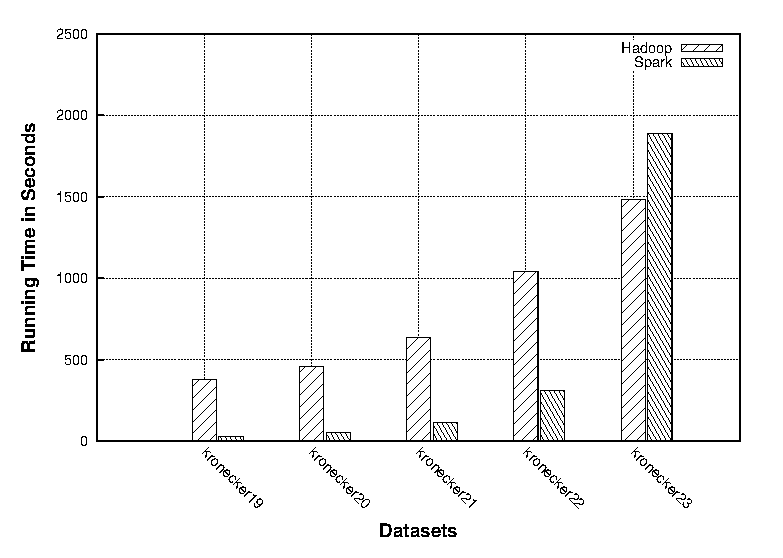
\includegraphics[width=0.4\textwidth]{figures/synthetic-5iterations-time.eps}}
\caption{Running time comparison.}
\label{fig:hadoopsparkrunningtime}
\end{figure*}

Fig. \ref{fig:hadoopsparkrunningtime} shows running time comparison between Hadoop and Spark using real and synthetic graph datasets. We have the following five observations. 

1) When dataset is too small, e.g., wiki-Vote, soc-Slashdot0902, Spark can outperform Hadoop by 25x-40x. In this case, the computing resources of all the slaves are underutilized. For Spark, it is the iterative computation time that dominates the total running time. But for Hadoop, it is the job initialization time, disk access time, I/O time and network communication time that contribute the major cost.   %So Spark has a great advantage over Hadoop.
%(For Hadoop one iteration takes two jobs, whereas for Spark, all iterations resides in one job.)

2) When dataset is relatively small, e.g., web-Google, kronecker19, kronecker20, Spark can outperform Hadoop by 10x-15x. In this case, the computing resources of all the slaves are moderately utilized. The iterative computation time begins to dominate the total running time of Hadoop and Hadoop starts to show its true performance.

3) When dataset is relatively large, e.g., cit-Patents, kronecker22, the advantage of Spark becomes small and Spark can only outperform Hadoop by 3x-5x. In this case, for Hadoop the memory of each slave in the cluster is still moderately utilized while for Spark the memory of each slave in the cluster is full (i.e. reaching the memory limit of each slave in the cluster) which result in Spark's reduced performance advantage.

4) When dataset is too large, e.g., kronecker23, Hadoop beats Spark. In this case, for Hadoop, the memory of each slave in the cluster is fully utilized while for Spark the memory of each slave in the cluster is not enough for PageRank running. There is no memory space for the newly created RDDs, so Spark starts its RDD replacement policy. Frequent RDD replacements cause Spark's performance to degrade to that of Hadoop, or even worse.  

5) When dataset is extremely large, e.g., Twitter, PageRank on Spark crashes halfway with JVM heap exceptions while PageRank on Hadoop can still run.


%From the next subsection, we can see that Spark is memory costly due to its memory based feature. 
%All the four cases show that iteration times of both platforms have large variance and a great degree of fluctuation. This involves a lot of influence factors, such as machine hardware differences, network status differences, unexpected task failures and so on.
%In case 1, where the dataset is wiki-Vote, Spark outperforms Hadoop by 47x. In case 2, where the dataset increases to soc-Slashdot0902, Spark's performance advantage reduces to 39x. By comparing the running time of Hadoop and Spark in Case 1 and 2, we find that when the dataset size doubles, the iteration time of Spark doubles too, but the iteration time of Hadoop does not. This is because in Case 1 the dataset is too small, for Hadoop it is the job initialization time and network communication time not the iterative computation time that dominates the iteration time, whereas for Spark it is the iterative computation time that dominates the iteration time. (For Hadoop one iteration takes one job, whereas for Spark, all 10 iterations resides in one job.) In Case 3, where the dataset increases to 015g, Spark's performance advantage reduces to 9.2x. This is not only because of the reason mentioned above, but also because of that reason that Spark has reached the memory litmit of the cluster and memory has become a bottleneck.

% averaging total running time is meanningful, whereas averaging each iteration running time is meaningless
% In order to eliminate the randomness of a single running of PageRank on Hadoop and Spark, we repeat 10 times running of PageRank on both platforms against three sizes of datasets and get averaged total running times. Fig. \ref{fig:iter10avgtime} shows the averaged value comparison of Hadoop and Spark.

\subsection{Memory Usage Comparison}

 By comparing memory usage plots of all the seven slaves, we find that their plots are roughly the same. This is because of the uniform distribution of the input data on the seven slaves and the load balancing strategy adopted by both Hadoop and Spark. So we will only illustrate the results for one slave (slave1), shown in Fig. \ref{fig:time_memory_real} and Fig. \ref{fig:time_memory_syn}. In each plot, memory occupancy over time for different graph datasets are shown by different curves in different colors.
%we find that for a specific dataset the memory usage plots of PageRank implementations on Hadoop and Spark on each slave are roughly the same.
 
\begin{figure*}[!t]
  \centering
  \subfloat[Hadoop]{    
    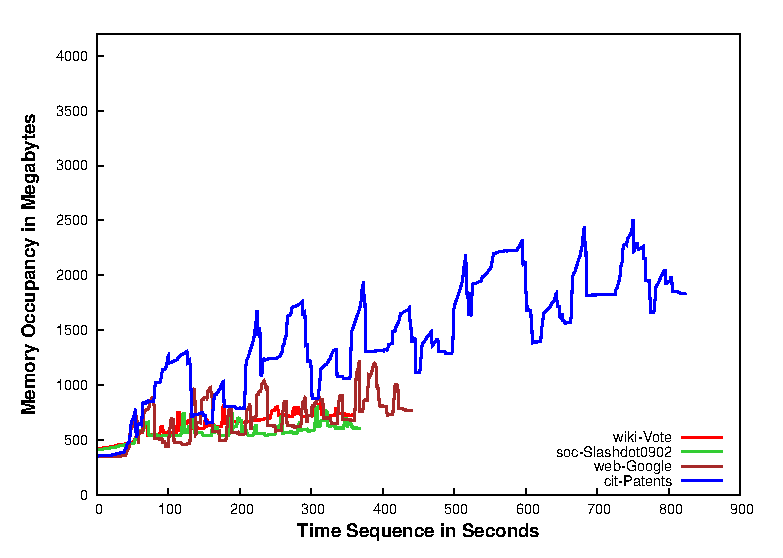
\includegraphics[width=0.4\textwidth]{figures/hadoop-real-time-memory.eps}}
  \subfloat[Spark]{ 
    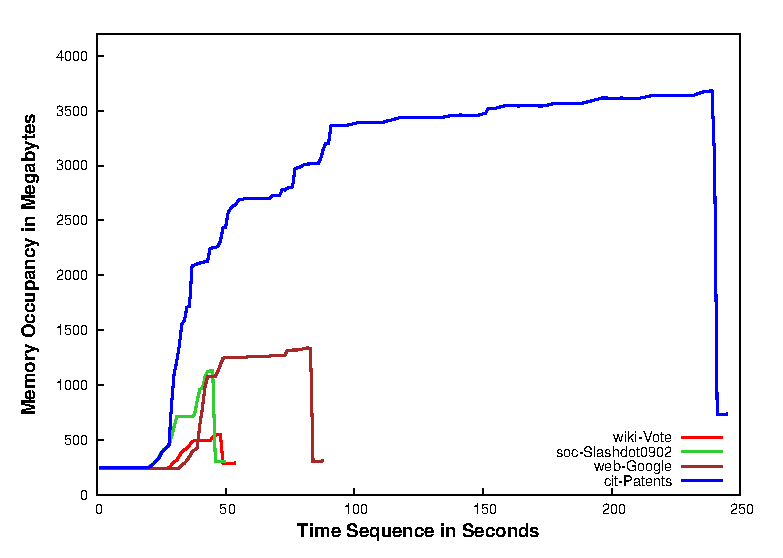
\includegraphics[width=0.4\textwidth]{figures/spark-real-time-memory.eps}}
  \caption{Memory usage comparison using real graph datasets.}
  \label{fig:time_memory_real} 
\end{figure*}

\begin{figure*}[!t]
  \centering
  \subfloat[Hadoop]{    
    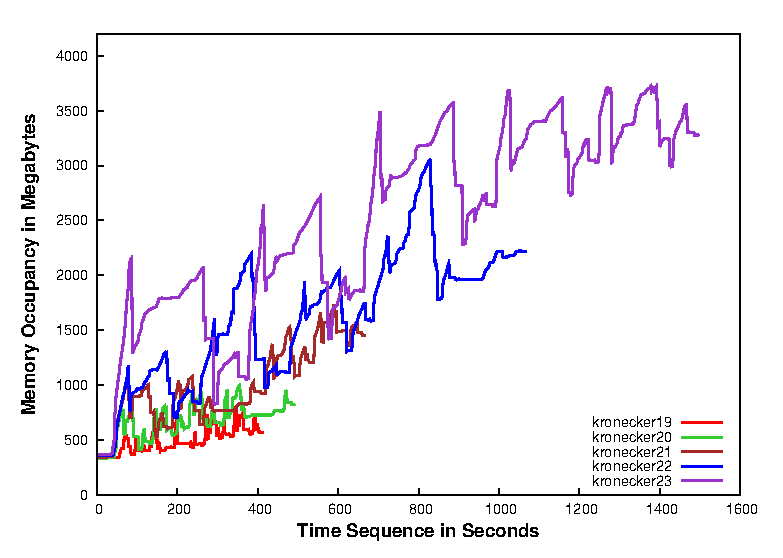
\includegraphics[width=0.4\textwidth]{figures/hadoop-synthetic-time-memory.eps}}
  \subfloat[Spark]{ 
    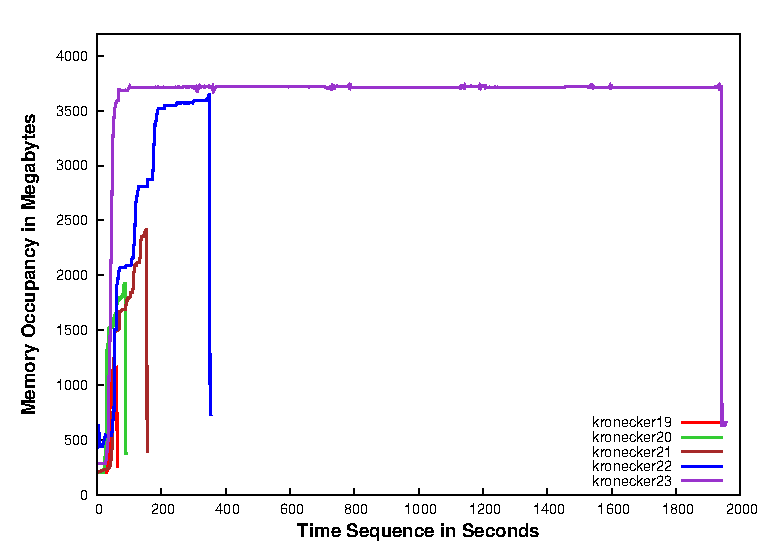
\includegraphics[width=0.4\textwidth]{figures/spark-synthetic-time-memory.eps}}
  \caption{Memory usage comparison using synthetic graph datasets.}
  \label{fig:time_memory_syn} 
\end{figure*}

For Hadoop platform, when dataset is fixed, memory usage exhibits periodically increase and decrease with the increase in the number of iterations. There is also a gradual increment between two consecutive iterations. The periodicity is due to the iterative nature of PageRank algorithm. Each cycle corresponds to one iteration of PageRank. In each cycle, there are three peaks, which corresponds to the Map and Reduce stages in the first job and the Map stage in the second job respectively. All these three stages consume memory and lead to a peak of memory usage. The Map stage in the first job comsumes a little bit more memory than its corresponding Reduce stage in the first job and Map stage in second job. Reduce stage in the first job lasts longer than the other two stages. 
%The gradual increase in memory usage between two consecutive iterations is probably due to the memory cache policy used by the operating system on which the Hadoop platform runs.

For Hadoop platform, when iteration number is fixed, the shapes of memory usage plots are similar with the increase in the size of dataset. Differences exist in two aspects. When dataset size is larger, the gradual increment between two consecutive iterations is bigger and the three peaks in each iteration are higher. When the increment reaches memory limit of a slave, the increase stops and the height of the three peaks does not change.

For Spark platform, when dataset is fixed, memory usage only exhibits periodically gradual increase with the increase in the number of iterations. The reason for periodicity is the same as that for Hadoop. However, there are no peaks in each cycle. The gradual increment between two consecutive iterations is because of the creation of new auxiliary RDDs. Spark uses RDD for data cache and RDD is a read-only data structure. There are two main RDDs in Spark's PageRank implementation. One is used for caching the graph structure, which will not change during iterative process. We call this RDD the main RDD. The other one is used for caching temporary PageRank value for each node in the graph, which will change in each iteration. We call this RDD the auxiliary RDD. Because of the read-only nature of RDD, a new auxiliary RDD will be created when changes happen to it in each iteration.

For Spark platform, when iteration number is fixed, the shapes of memory usage plots are similar with the increase in the size of dataset. When dataset size is larger, the gradual increment between two consecutive iterations is bigger. When the increment reaches memory limit of a slave, the increase stops. When the dataset size is too large, the program cannot run without enough memory.

In Hadoop platform, iterative operations are implemented through multiple MapReduce computations. Each iteration corresponds to one or more MapReduce computations. When a Map or Reduce computation ends, the memory used by it will be released. Whereas, in Spark platform, iterative operations are implemented in a single Spark program. So there is no memory release phenomenon in Spark implementation. 

From the experimental memory plots, we can also find that Spark is extremely memory consuming. For a graph dataset whose size is 300M-500M, the total 21GB memory of the cluster will be occupied. 


% \begin{table*}[!t]
% \renewcommand{\arraystretch}{1.3}
% \centering
% \begin{tabular}{|c|c|c|c|}
% \hline
% \bfseries Name & \bfseries Hadoop & \bfseries Spark & \bfseries Ratio\\
% \hline
% wiki-Vote & 337s & 9s & 37.4 \\
% \hline
% soc-Slashdot0902 & 330s & 13s & 25.4\\
% \hline
% web-Stanford & 349s & 23s & 15.2 \\
% \hline
% web-Google & 407s & 51s & 7.98\\
% \hline
% web-BerkStan & 458s & 47s & 9.7 \\
% \hline
% cit-Patents & 796s & 197s & 4.04\\
% \hline
% \end{tabular}
% \caption{Hadoop and Spark scalability experiment with 7 slaves using real graphs}
% \label{tab:hadoop_spark_scala_7slaves_realgraph}
% \end{table*}


% \begin{table*}[!t]
% \renewcommand{\arraystretch}{1.3}
% \centering
% \begin{tabular}{|c|c|c|c|}
% \hline
% \bfseries Name & \bfseries Hadoop & \bfseries Spark & \bfseries Ratio\\
% \hline
% kronecker19 & 379s & 30s & 12.6\\
% \hline
% kronecker20 & 457s & 55s & 8.3\\
% \hline
% kronecker21 & 637s & 117s & 5.4\\
% \hline
% kronecker22 & 1040s & 311s & 3.3\\
% \hline
% kronecker23 & 1481s & 1888s & 0.78\\
% \hline
% \end{tabular}
% \caption{Hadoop and Spark scalability experiment with 7 slaves using synthetic graphs generated by Kronecker generator.}
% \label{tab:hadoop_spark_scala_7slaves_syngraph}
% \end{table*}

% \begin{figure*}[!t]
%   \centering
%     \subfloat[Real Graphs]{
%         \includegraphics[width=0.5\textwidth]{time/hadoop-spark/7-slaves/real/hadoop-low-high.eps}}
%     \subfloat[Synthetic Graphs]{
%         \includegraphics[width=0.5\textwidth]{time/hadoop-spark/7-slaves/synthetic/hadoop-low-high.eps}}
%   \caption{Running time comparison among Hadoop-0.20.205.0, Hadoop-1.1.2 and Spark on real graphs and synthetic graphs. For each dataset, we make both implementations of PageRank iterate 5 times and record total time spent.}
%   \end{figure*}

% An example of a floating figure using the graphicx package.
% Note that \label must occur AFTER (or within) \caption.
% For figures, \caption should occur after the \includegraphics.
% Note that IEEEtran v1.7 and later has special internal code that
% is designed to preserve the operation of \label within \caption
% even when the captionsoff option is in effect. However, because
% of issues like this, it may be the safest practice to put all your
% \label just after \caption rather than within \caption{}.
%
% Reminder: the "draftcls" or "draftclsnofoot", not "draft", class
% option should be used if it is desired that the figures are to be
% displayed while in draft mode.
%
%\begin{figure}[!t]
%\centering
%\includegraphics[width=2.5in]{myfigure}
% where an .eps filename suffix will be assumed under latex, 
% and a .pdf suffix will be assumed for pdflatex; or what has been declared
% via \DeclareGraphicsExtensions.
%\caption{Simulation Results}
%\label{fig_sim}
%\end{figure}

% Note that IEEE typically puts floats only at the top, even when this
% results in a large percentage of a column being occupied by floats.


% An example of a double column floating figure using two subfigures.
% (The subfig.sty package must be loaded for this to work.)
% The subfigure \label commands are set within each subfloat command, the
% \label for the overall figure must come after \caption.
% \hfil must be used as a separator to get equal spacing.
% The subfigure.sty package works much the same way, except \subfigure is
% used instead of \subfloat.
%
%\begin{figure*}[!t]
%\centerline{\subfloat[Case I]\includegraphics[width=2.5in]{subfigcase1}%
%\label{fig_first_case}}
%\hfil
%\subfloat[Case II]{\includegraphics[width=2.5in]{subfigcase2}%
%\label{fig_second_case}}}
%\caption{Simulation results}
%\label{fig_sim}
%\end{figure*}
%
% Note that often IEEE papers with subfigures do not employ subfigure
% captions (using the optional argument to \subfloat), but instead will
% reference/describe all of them (a), (b), etc., within the main caption.


% An example of a floating table. Note that, for IEEE style tables, the 
% \caption command should come BEFORE the table. Table text will default to
% \footnotesize as IEEE normally uses this smaller font for tables.
% The \label must come after \caption as always.
%
%\begin{table}[!t]
%% increase table row spacing, adjust to taste
%\renewcommand{\arraystretch}{1.3}
% if using array.sty, it might be a good idea to tweak the value of
% \extrarowheight as needed to properly center the text within the cells
%\caption{An Example of a Table}
%\label{table_example}
%\centering
%% Some packages, such as MDW tools, offer better commands for making tables
%% than the plain LaTeX2e tabular which is used here.
%\begin{tabular}{|c||c|}
%\hline
%One & Two\\
%\hline
%Three & Four\\
%\hline
%\end{tabular}
%\end{table}




% Note that IEEE does not put floats in the very first column - or typically
% anywhere on the first page for that matter. Also, in-text middle ("here")
% positioning is not used. Most IEEE journals/conferences use top floats
% exclusively. Note that, LaTeX2e, unlike IEEE journals/conferences, places
% footnotes above bottom floats. This can be corrected via the \fnbelowfloat
% command of the stfloats package.
\section{Related Work}
\label{sec:related_work}

MapReduce is first proposed by Dean and Ghemawat in \cite{jdean2004}. As a new programming model, MapReduce is suitable for processing and generating large data sets in a scalable, reliable and fault-tolerant manner. Apache Hadoop\cite{url_hadoop} provides an open source implementation of MapReduce. Performance of MapReduce has been deeply studied in \cite{jiang2010}\cite{lee2012}. In their results, the authors show that with proper implementation, performance of MapReduce can approach traditional parallel databases while achieving scalability, flexibility and fault-tolerance. However, Hadoop shows poor performance in iterative operations which are very common in many data analysis techniques.

Spark\cite{matei2010} was developed recently to optimize iterative and interactive computation. It uses caching techniques to dramatically improve the performance for repeated operations. The main abstraction in Spark is called $resilient\;distributed\;dataset$ (RDD), which is maintained in memory across iterations and fault tolerant. Spark can outperform Hadoop by 10x in iterative machine learning jobs, and can be used to interactively query a 39 GB dataset with sub-second response time. Other similar works include Twister\cite{jaliya2010} and HaLoop\cite{yingyi2010}. Compared with Hadoop, Twister outperforms Hadoop in parallel efficiency; HaLoop averagely reduces query runtimes by 1.85, and shuffles only 4\% of the data between mappers and reducers.

Some efforts focus on iterative graph algorithms, an important class of iterative algorithms. Pegsus\cite{kang2009} unifies many iterative graph algorithms as Generalized Iterated Matrix-Vector multiplication (GIM-V). By exploiting special properties of matrix, it can achieve more than 5x faster performance over the regular version. Pregel\cite{malewicz2010} chooses a pure message passing model to process graphs. In each iteration, a vertex can, independent of other vertices, receive messages sent to it in the previous iteration, send messages to other vertices, modify its own and its outgoing edges' states, and mutate the graph's topology. By using this model, processing large graphs is expressive and easy to program. Distributed GraphLab\cite{low2012} is similar to Pregel. The key difference between Pregel and GraphLab is that Pregel has a barrier at the end of every iteration, whereas GraphLab is completely asynchronous. Experiments show that applications created using Distributed GraphLab outperform equivalent Hadoop/MapReduce implementations by 20-60x.


\section{Conclusions and Future Work}
\label{sec:concl_fw}

For different experiment settings,  we find that although Spark is in general faster than Hadoop, it is at the cost of significant memory consumption. If speed is not a demanding requirement and we do not have abundant memory, it's better not choose Spark.  In this case, as long as we have enough disk space to accommodate the original dataset and intermediate results, Hadoop is a good choice.

For a specific iterative operation, if the application is time sensitive, Spark should be considered. But  enough memory is a necessary condition for the operation in order to secure Spark's performance advantage. The problem is that it is hard to determine the accurate amount of memory for iterative operations running on Spark. Exactly how much memory is enough depends on the particular iterative algorithm and the size of the dataset it processes. Intermediate results during iterations are stored in memory as RDDs. Because of the read-only nature of RDD, new RDDs will always be created in each iteration. If the size of intermediate results is at constant level, the increase of memory usage between two consecutive iterations is not significant. If the size of the intermediate results is proportional to the size of the input dataset (like PageRank), the increase of memory usage between two consecutive iterations is significant.

As part of our future work, we plan to find a prediction model for the tradeoff of response time and memory usage for iterative operations. Also we will explore the influence of graph structures on response time of iterative operations.
%how to quantify the tradeoff in terms of time and memory for iterative operations
% conference papers do not normally have an appendix


% use section* for acknowledgement
\section*{Acknowledgement}
We would like to thank the Social Computing Data Repository at ASU\cite{zafarani2009} for providing us the Twitter graph dataset\cite{url_twitter_dataset}. 

This work is supported by a grant from the National High Technology Research and Development Program of China (2012AA0011203); the Scientific Research Foundation for the Returned Overseas Chinese Scholars, State Education Ministry; and State Key Laboratory of Software Development Environment (SKLSDE-2012ZX-03).

% trigger a \newpage just before the given reference
% number - used to balance the columns on the last page
% adjust value as needed - may need to be readjusted if
% the document is modified later
%\IEEEtriggeratref{1}
% The "triggered" command can be changed if desired:
%\IEEEtriggercmd{\enlargethispage{-5in}}

% references section

% can use a bibliography generated by BibTeX as a .bbl file
% BibTeX documentation can be easily obtained at:
% http://www.ctan.org/tex-archive/biblio/bibtex/contrib/doc/
% The IEEEtran BibTeX style support page is at:
% http://www.michaelshell.org/tex/ieeetran/bibtex/
\bibliographystyle{IEEEtran}
% argument is your BibTeX string definitions and bibliography database(s)
\bibliography{IEEEabrv,references}
%
% <OR> manually copy in the resultant .bbl file
% set second argument of \begin to the number of references
% (used to reserve space for the reference number labels box)
% that's all folks
\end{document}